\chapter{Introduction}
\label{ch:introduction}

\section{Motivation \& Problem Statement}
\label{sec:motivation}
In the last years the demand of information availability and shorter response times is increasing.
Existing problems, such as the large amount of data to process and analyze in a big data application, are not the only challenges to solve.
There are many sensors, mobile devices and other IoT devices out in the field, constantly sending data in form of streams to the processing servers.\\
Today's business requirements are changing: Waiting hours or even days for the result of a query is not acceptable anymore in many sectors.
The response needs to be immediate, or the query is discarded \cite{estrada2016big}.
Quick responses, ideally near real-time, are crucial success factors.
Many data warehouses are facing the problem that the stored data is slowly becoming obsolete.
This is why "Fast Data", as an approach to solve those problems, increases its popularity, as being "big data, but fast" \cite{mishne2013fast}. \\


The SMACK-Stack consists of five technologies combined to a lightning fast data pipeline for today's needs of big data applications.\\
\begin{itemize}
    \item Apache \textbf{S}park is the engine of the pipeline, providing batch-, as well as stream-processing power for large-scale data processing.
    \item \textbf{M}esos is a datacenter operating system with the aim to reduce complexity and ease the deployment and maintenance of large-scale distributed applications.\\
    \item Apache \textbf{A}kka can be seen as the model, providing the possibility to build powerful reactive distributed message-driven applications.\\
    \item Apache \textbf{C}assandra is a highly distributed database which is a hybrid between a column-oriented and a key-value DBMS, which is implemented avoiding a single point of failure.\\
    \item Apache \textbf{K}afka serves as publish-subscribe message broker, which is usually the ingestion point of the pipeline.\\
\end{itemize}


\section{Motivating Scenarios}
To evaluate the framework developed in the course of this thesis, an extensive evaluation is performed.
The setup contains two real world applications, which serve as a basis for benchmarking and exploring the optimal resource distribution when scaling up and down.
One application is I/O-bound, which means there is not a lot of logic inside the data pipeline, but many requests have to be processed, which is done with real world IoT data.
The other one is a computational bound application, which does not have to deal with many requests in parallel but requires a lot of computation power inside the pipeline.

\subsection{Real World IoT Data Storage Application}
\label{sec:iot_application}
During the HackZurich 2016 \cite{hackzurich_website}, Europe's largest hacking contest, Zuehlke Engineering AG \cite{zuehlke} developed a simple real world IoT application to be used with SMACK \cite{hackzurich}.\\
The application can be categorized as sensor data ingestion and analysis software.
It is designed to run in a cluster and handle vast amounts of incoming data.\\
As this is the product of a hackathon, the initial state was only a very basic implementation and had to be extended to fit the needs of this thesis.\\

In abstract terms, the application serves as endpoint for ingesting and storing relevant IoT data.
The devices connect and send their data via HTTP to a REST endpoint.
After this, the data pipeline processes and normalizes the input to finally store the data into the Cassandra database for later analysis or statistical evaluation.\\

Figure~\ref{fig:hackzurich} gives a rough overview of how the single components of SMACK are interacting with each other in this application.
In Figure~\ref{fig:iot} a more detailed view gives insight of how the application is designed.\\
All the IoT devices are sending their data in JSON the REST webservice named \textit{sensor-ingestion}, implemented using Akka actors.
The reason to use Akka is to be able to provide a reactive application without a lot of manual programming effort.
While the JSON input is not parsed in Akka it is simply transferred to a Kafka topic - in this case to the topic \textit{sensor-reading} - to be processed later on in Spark.\\
This means that Kafka servers as a buffer here to allow the ingestion to be decoupled from the processing.
In the Spark job, which is called \textit{KafkaToCassandra}, the JSON is parsed and validated and then send to Cassandra to be stored in the \textit{sensordata} keyspace for later analysis.\\

A handy tool to interact with Cassandra and to perform real-time data analysis, is Apache Zeppelin, which provides interactive scratch books and can be used with most modern big data technologies.
There are some example scratch books in the repository, which can be used in the context of the sensor data application.\\

All commits can be found in the repository \cite{hackzurich}, but the main contribution to this application can be summarized in the following points:
\begin{itemize}
    \item Fixing compile errors and updating dependencies
    \item Updating docker image creation
    \item Collecting and computing statistics / metrics for the application
    \item Adding a feature to export metrics of the sensor ingestion via JMX
    \item Extension of the existing load generator.\\
          The JSON files are now compacted to be able to achieve higher throughputs and use less CPU on the client side.
          Further the input handling of those files had to be adjusted.
\end{itemize}

The application can be categorized as real world application, because real IoT sensor data has been recorded and can be used again for later stress testing.
Further the scenario is not artificial - in the context of the HackZurich, a company producing and maintaining elevators used this application to gather information about their products to use it for predictive maintenance.\\
As it can be seen from the context of the application, consistency in terms of not losing a single sensor data is not required.
It is required though, that the system stays reactive and responsive even under heavy load and is capable of handling the data in a fault-tolerant way.
For example if one node goes offline, the whole data pipeline must not be disturbed, as it would mean that data loss occurs.
Further the persistence is a highly desired property in this scenario.
The data must be stored securely, so that the data scientists can later on perform their analysis for the predictive maintenance, even when the stack goes offline.

\begin{figure}[!htbp]
  \centering
  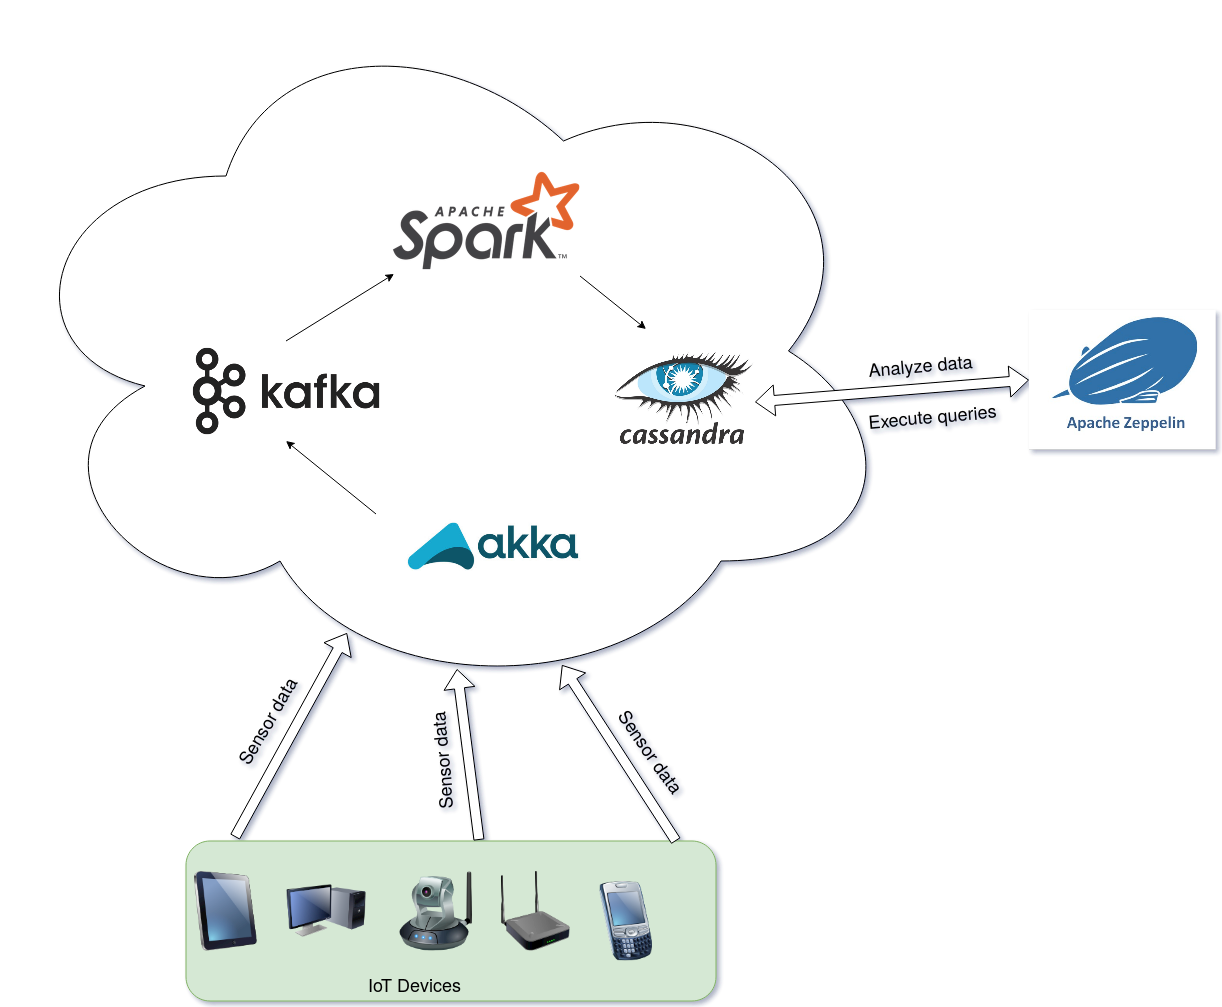
\includegraphics[keepaspectratio=true,scale=0.38]{img/hackzurich}
    \caption{Abstract View of Zuehlke HackZurich IoT Application}
  \label{fig:hackzurich}
\end{figure}

\begin{figure}[!htbp]
  \centering
  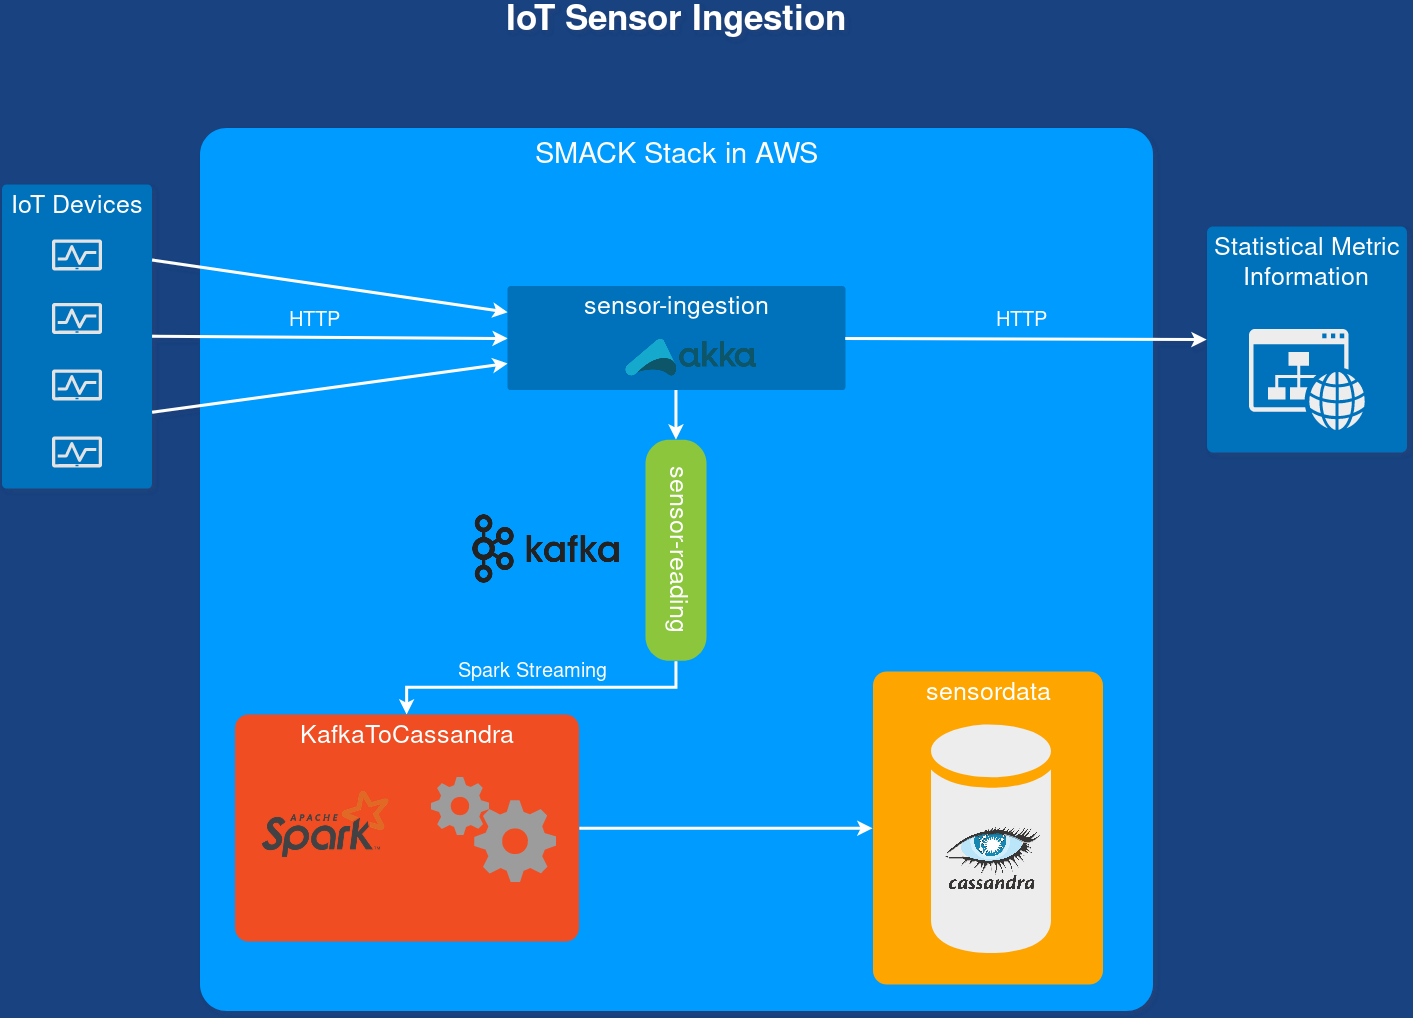
\includegraphics[keepaspectratio=true,scale=0.35]{img/IoT}
    \caption{Detailed View of the Zuehlke HackZurich IoT Application}
  \label{fig:iot}
\end{figure}


\subsection{Real World Acceleration Prediction Application}
\label{sec:computation_application}
In the course of this thesis, a new application was developed which is mainly computational bound and handles less input data than the IoT application.
The IoT application is used as a base, including the real life data, but as mentioned, just a fraction of the volume is ingested.\\
Information about how the data looks like in detail can be found in section \ref{sec:sensor-data}.\\

To provide a realistic use case, this application learns from the past and predicts the movements of the elevators in the future.
This could be especially helpful when talking about predictive maintenance or even more when optimizing the idle time of the elevators.
Imagine the waiting times at an elevator can be reduced because it automatically starts to move up or down based on the prediction.
In most cases, the elevator would be in movement even before the real request by a user would occur.\\
The application is written in Scala and Spark using an ARIMA model of the spark-timeseries library.
Information about the history is gathered from the Cassandra database, which is filled with data by using the light-weighted version of the IoT application.\\

Figure~\ref{fig:prediction} illustrates the architecture of the whole application.\\
As one can see, the ingestion part is the same as in the IoT application as mentioned above.
The data is ingested by the \textit{sensor-ingestion} application based on Akka, which writes in the \textit{sensor-reading} Kafka topic.
From there the \textit{KafkaToAccelerometer} Spark job constantly receives data via Spark Streaming and writes the processed data into the \textit{sensordata} keyspace of Cassandra, as well as publishing the latest processed accelerometer data into the \textit{sensor-reading-accelerometer} Kafka topic.\\
The \textit{Prediction Data Analytics} Spark job constantly polls from Cassandra and calculates the predictions based on the available data.
The results are written into the \textit{data-analytics} topic.
In the \textit{akka-data-analytics} application the results of the slower but more precise prediction from Spark are polled.
Additionally the application performs a basic prediction with the help of linear regression, based on the available data from the \textit{sensor-reading-accelerometer} topic.\\
This design is related to the Lambda architecture, which uses a speed and a batch layer, to be able to constantly provide results to the end user.
In the application, both predictions are combined if available.
If there is just data from the "speed layer" or just the "batch layer" this data is published via HTTP to the end user.
In case both layers provide data for the same timestamp, the values are combined with the help of weights, ${speed} * 0.3 + {batch} * 0.7$.\\

In order to generate a satisfying amount of datasets the application only considers \textit{Accelerometer} data, as this data occurrs most frequently in the real-life dataset.
Additionally the information about the acceleration is enough to provide predictive values of when the elevator should start to move up or down.

\begin{figure}[!htbp]
  \centering
  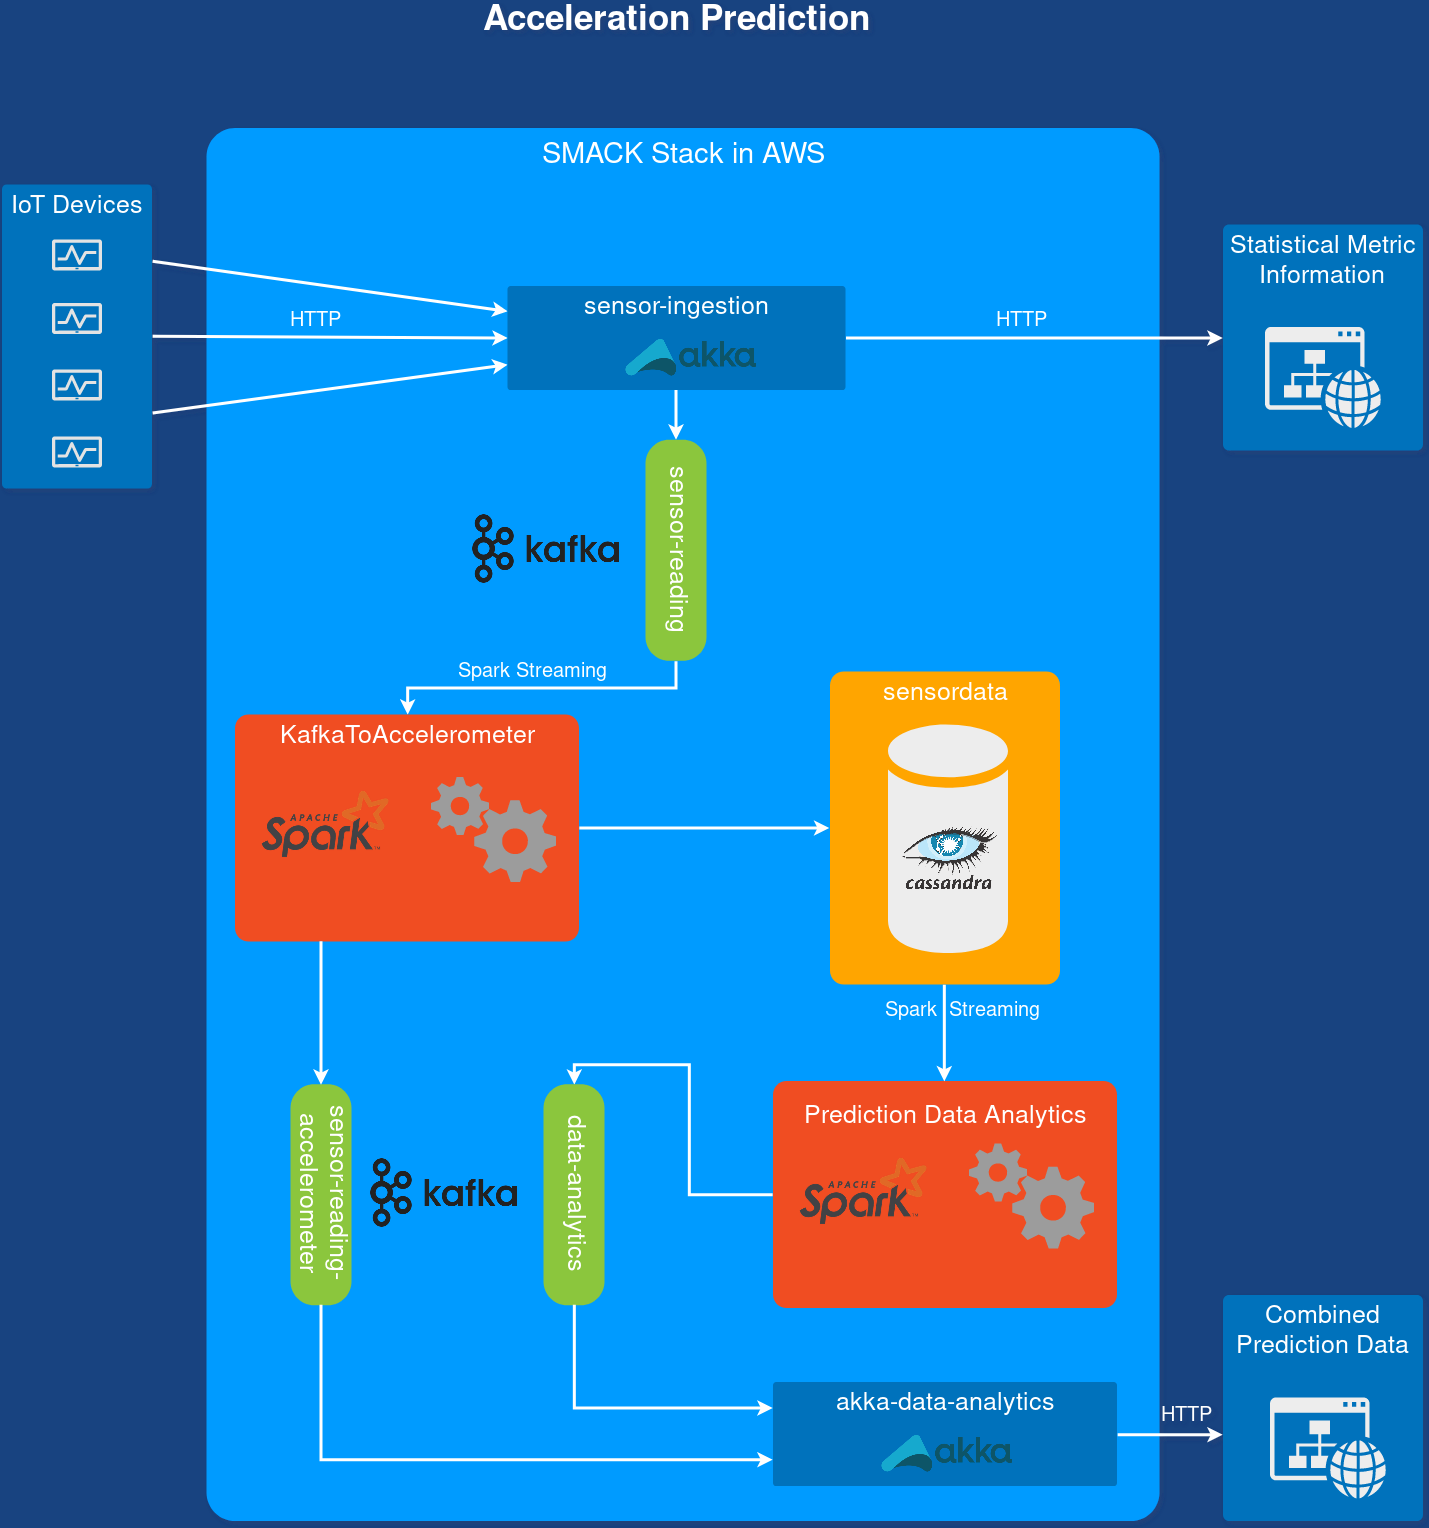
\includegraphics[keepaspectratio=true,scale=0.33]{img/prediction}
    \caption{Detailed View of the Acceleration Prediction Application}
  \label{fig:prediction}
\end{figure}


To measure the quality of the predictions, a \textit{Kolmogorov Smirnov Test} is done \cite{wilcox2005kolmogorov}.
The setup of the test looks like follows:\\
\begin{enumerate}
    \item Select only those values for which a prediction and the real value is given for the same timestamp (and obviously the same elevator/device).
    \item Accumulate the values of the dataset, where $x$ are the timestamps and $y$ are corresponding values.\\
          $c_1 = y_1$\\
          $c_2 = c_1 + y_2$\\
          $c_n = c_{n-1} + y_n$\\
          ...
    \item Create a new dataset which consists of the same x-values and for each y-value calculate $y_{diff} = abs(y_{real} - y_{prediction})$.
    \item Now we can calculate the minimum, maximum and average of the differences and add this curve to the plot.
\end{enumerate}

For an easy and illustrative comparison of the real versus the predicted data, the Kolmogorov Smirnov Test is plotted in Figure~\ref{fig:prediction_vs_real}, where the following statistical values apply with respect to the calculated difference-curve:\\
${Min}: 0.04$\\
${Max}: 8.56$\\
${Avg}: 5.05$\\

The K.S. Test indicates that the prediction is promising.
One can observe that the curves develop very similar but are a bit biased.
The compensation or removal of this bias could be a possible further improvement for future work.
Still the K.S.-Test confirms, that the prediction is not "random output" and has a measurable correlation to the real values.

\begin{figure}[!htbp]
  \centering
  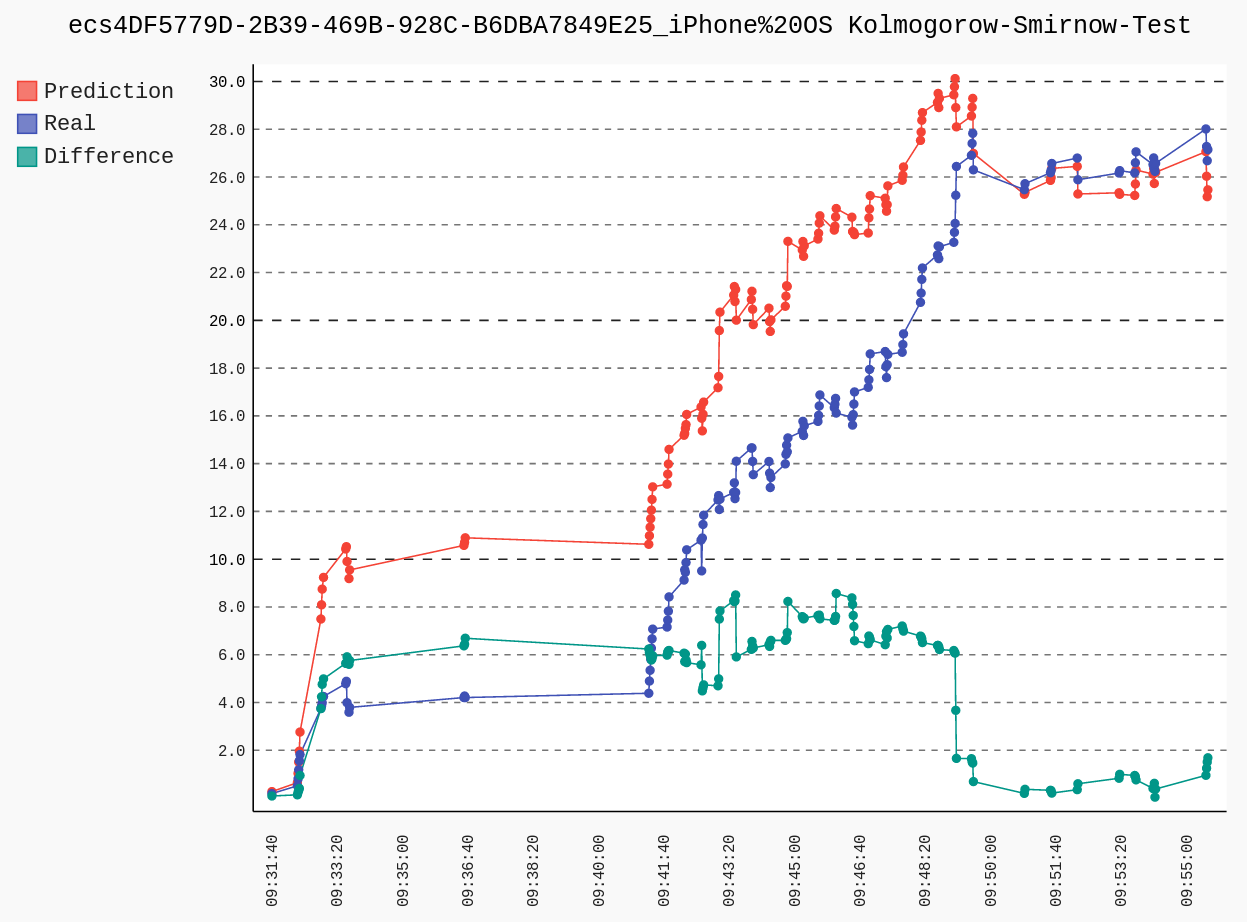
\includegraphics[keepaspectratio=true,scale=0.36]{img/prediction_vs_real}
    \caption{Kolmogorov Smirnov Test - Prediction versus Real}
  \label{fig:prediction_vs_real}
\end{figure}


\section{Research Challenges}
In terms of operating and managing a cluster there are a various challenges, developers and system administrators are faced with.\\
\begin{itemize}
    \item Deploying large scale applications\\
          When facing the challenge of deploying productive applications in a large scale cluster, several factors need to be considered.
          Many applications consist of multiple instances of different technologies, or are hosted in various Docker containers.
          The deployment needs to be performed in a defined sequence to fulfill subsequent dependencies.
          In addition, depending on the used cluster manager, a lot of manual steps are required until the application is ready and online.
    \item Initial setup\\
          The decision of how to configure the instances of an application is a non-trivial task, as there are almost infinite combination possibilities and the impact can be drastic.
          Finding the right distribution of resources within a cluster across the hosted applications can be a challenging task.
          This is especially crucial when the deployed application deals with large amounts of data and clients, while still staying responsive and fault-tolerant.
    \item Monitoring\\
          There are many tools available to monitor clusters and big data applications, although a deeper understanding of the used frameworks is required.
          Considering just RAM, CPU and disk usage is in most cases insufficient.
          For example, a high usage of RAM in a Spark Job would not necessarily mean that it is under heavy load, but that Spark uses - per design - a lot of memory to leverage it's computation power, compared to disk intensive frameworks like Hadoop.
          This introduces a new layer of complexity, as each framework has its own characteristics and metrics to observe when monitoring a cluster.
          Understanding what's going on in a cluster and reacting accordingly is crucial for the success of any large scale application.
    \item Scaling when needed\\
          Recognizing when to scale which component of an application is a 24/7 task.
          In the ideal case, the system automatically scales up and down as required.
          There are many existing approaches, but the quality of the automated scaling still relies heavily on the quality and significance of the monitored metrics.
          Without the right metrics, the scaling cannot be reliable and thus requires most of the time manual decisions.
\end{itemize}

All the components of the SMACK stack proved that they are very scalable used in isolation.
Now the question is, where is the bottleneck when using them as combined data pipeline?
Another important question is how to distribute the resources in an optimal way.
For example if there is an application running in the cloud, how should the CPU, RAM, disk space etc. be assigned to the different technologies to achieve the best performance for the lowest price.
Of course this question can only be answer with respect to the requirements of the application and the kind of data to process, i.e. the input data pattern.
This is where a framework can be developed to automatically analyze and regulate resource allocation for the SMACK stack.\\


\section{Background}
This section givs an overview of the single components of the SMACK stack, namely Spark, Mesos, Akka, Cassandra and Kafka.
A basic knowledge of the used technologies is crucial for the reader to be able to understand the complex interdependencies which are omnipresent when using a big data stack with multiple technologies.

\subsection{Akka}
"Akka is a toolkit for building highly concurrent, distributed, and resilient message-driven applications for Java and Scala" \cite{akka_web}.\\
The mathematical model behind Akka is the \textit{Actor Model}, which was developed and presented in the first place by C. Hewitt, P. Bishop and R. Steiger in 1973 \cite{hewitt1973session}.
During the time the paper was written, hardware was very expensive, which is not the case anymore today.
As a consequence, implementing large scale systems processing millions of requests per second is now possible in a cheap fashion.\\

One can imagine actors as objects which are receiving and sending messages between each other.
Because in theory the order of the messages is not relevant, the behavior of statelessly handling messages is encouraged.
The Akka implementation provides a so called \textit{mailbox}, in which messages are stored to be processed later in case an actor receives multiple messages at once.
These mailboxes usually have a limit after which newly received messages are simply dropped.
An actor can internally handle and process a message, but can also forward it to another actor, or even create a new actor to help achieving the required task.\\

According to the official Akka website, akka.io, the provided framework is the defacto-standard implementation of the actor model and comes with some interesting key features in aspect of big data \cite{akka_web}.
The framework is designed to be resilient by design, which allows developers to implement self-healing and responsive applications with ease.
Further the website claims to prodive capacity handling of 50 million messages per second on a single machine, while one GB of available heap can host up to 2.5 million actors.
This in combination with the asynchronous nature of the model provides a powerful platform to build responsive and highly scalable big data applications.


\subsection{Apache Spark}
"Apache Spark is a fast and general engine for large-scale data processing" \cite{apache_spark}. \\
Build for big data processing, this open-source framework offers the possibility outperform existing Hadoop solutions with ease.
"It has emerged as the next generation big data processing engine, overtaking Hadoop MapReduce which helped ignite the big data revolution.
Spark maintains MapReduce's linear scalability and fault tolerance, but extends it in a few important ways: it is much faster (100 times faster for certain applications)" \cite{shanahan2015large}.
The main reason for the immense speed is the build in direct acyclic graph execution engine, which supports in-memory computing, as well as acyclic data flows.\\

One big advantage of Spark is it's rich set of APIs, like Scala, Java, Python, R etc.
There are over 80 high-level operators, which allows developers to easily build robust and highly parallel applications.
For trying out new concepts or algorithms, there is an interactive mode, the so called Spark-shell. \\

In addition to the Spark core, there it consists of four main components:

\begin{itemize}
\item Spark SQL\\
This module allows the developer to work with structured data.
It provides seamless integration of Spark programs with SQL queries.
Another very powerful feature of Spark SQL is that one can uniformly access data, which means that there is just one common way to access all kind of supported data sources.
An example could be loading a JSON file is from Amazon S3 and used later as a table in an SQL query.\\
Further it is also possible to use JDBCS or ODBC drivers to connect ones business application to Spark.

\item Spark Streaming\\
The goal of this component is to provide both, fault-tolerance and scalability for streaming applications.
Through build-in high-level operators, it is possible to write streaming jobs in the same way one would implement a batch job.
A very powerful feature is the automatic recovery strategies - Spark recovers the state of the application as well as the lost worker node without requiring any additional code.
This is enables the developers to focus on what they want to implement on don't have to deal with complex fault tolerance for each component.\\
Again, it is possible to use the same code for batch, stream or ad-hoc queries, which leads to the possibility of building interactive applications without a lot of effort.

\item MLib\\
The integrated machine learning library provides many high quality algorithms, implemented to be efficient out of the box.
It's up to 100 times faster than traditional MapReduce approaches, such as Hadoop.
The dramatic runtime comparison difference can be seen in Figure~\ref{fig:spark_vs_hadoop}.


\begin{figure}[!htbp]
  \centering
  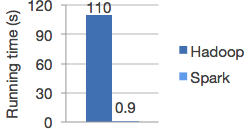
\includegraphics[keepaspectratio=true,scale=0.7]{img/spark_vs_hadoop}
    \caption{Spark vs. Hadoop - "Logistic regression in Hadoop and Spark" \cite{apache_spark}}
  \label{fig:spark_vs_hadoop}
\end{figure}

\item GraphX\\
    This API is designed to allow graph-parallel computation in combination with collections a seamless way.
    Thanks to the community the library of graph algorithms is growing and openly available for everyone.
    In terms of speed, the GraphX implementations can be compared with other state of the art graph libraries, which is illustrated in Figure~\ref{fig:spark_graphx}.

\begin{figure}[!htbp]
  \centering
  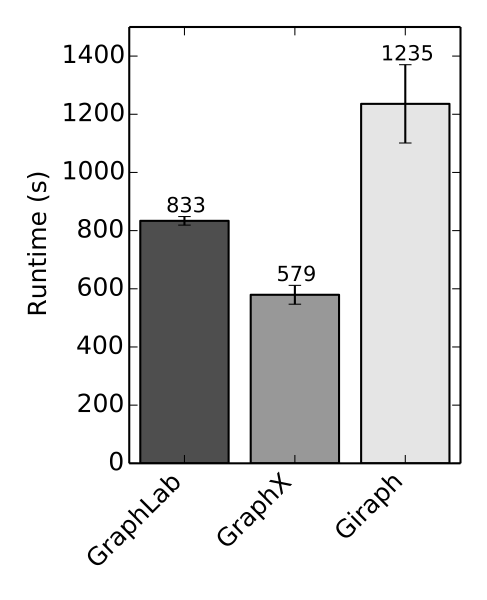
\includegraphics[keepaspectratio=true,scale=0.5]{img/spark_graphx}
    \caption{"End-to-end PageRank performance (20 iterations, 3.7B edges)" \cite{apache_spark}}
  \label{fig:spark_graphx}
\end{figure}

\end{itemize}

\textbf{Spark Architecture}\\
Figure~\ref{fig:spark_cluster_overview} illustrates the general architecture of any Spark program, regardless whether running in standalone or cluster mode.
The driver program is responsible for creating and executing operations on the so called Resilient Distributed Datasets (RDD), which are a main feature of Spark.
RDDs are abstractions of parallelized collections and have some powerful characteristic, especially when dealing with Big Data.
Those data structures are immutable, resilient, use lazy evaluation, are process aware and live in memory.\\
In addition, the driver is also responsible for creating and maintaining the Spark context, which is necessary for the connection between the nodes and the cluster.
Further configuration settings can be passed to the context during initialization, which affect the whole Spark program.
In our case, the cluster manager will be Mesos, which is responsible for launching and distributing the executors.\\
As the figure shows, each executor can run multiple tasks and usually in cluster mode, each executor is placed on a different worker node to provide even more fault-tolerance in case a node dies unexpectedly, but this behaviour can of course be overwritten manually.
If the driver node dies, the whole Spark program will be shutdown.
For this case a dedicated recovery strategy would have to be set up and implemented.

\begin{figure}[!htbp]
  \centering
  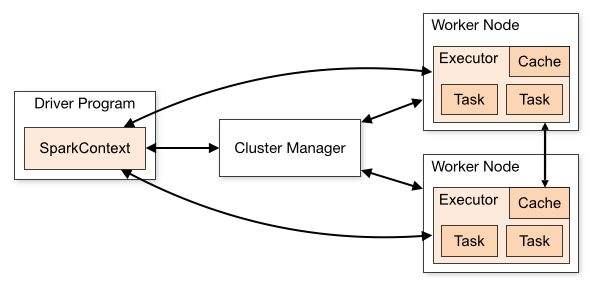
\includegraphics[keepaspectratio=true,scale=0.6]{img/spark_cluster_overview}
    \caption{Spark cluster with two executor nodes \cite{apache_spark}}
  \label{fig:spark_cluster_overview}
\end{figure}


\subsection{Apache Cassandra}
"Apache Cassandra is a free and open-source distributed NoSQL database management system designed to handle large amounts of data across many commodity servers, providing high availability with no single point of failure" \cite{cassandra_wikipedia}.\\
Many big companies, like eBay, Netflix, GitHub, etc. rely on the power of Cassandra to manage and store their data.
The masterless design offers flexibility as the cluster can be scaled up and down without any down time.
In Cassandra, the key-value and column oriented approach is combined to achieve extra performance when reading and writing data.\\
Research has been done concerning the speed of Cassandra: "In terms of scalability, there is a clear winner throughout our experiments.
Cassandra achieves the highest throughput for the maximum number of nodes in all experiments with a linear increasing throughput from 1 to 12 node" \cite{rabl2012solving}.\\
Due to the automatic replication of data onto multiple nodes, fault-tolerance is ensured.
In addition there is also support for replication across data center.\\
Cassandra comes with a custom Cassandra Query Language (CQL), which was designed to be close to what most developers know very well - regular SQL.

\begin{figure}[!htbp]
  \centering
  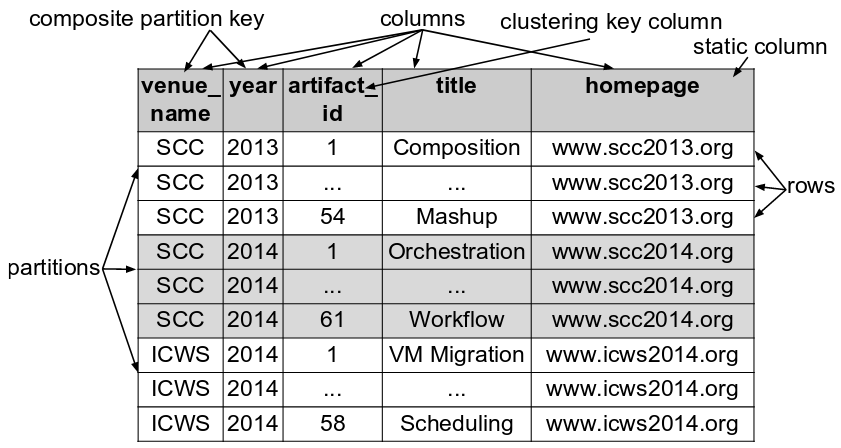
\includegraphics[keepaspectratio=true,scale=0.4]{img/cassandra_table}
    \caption{Cassandra Table \cite{chebotko2015big}}
  \label{fig:cassandra_table}
\end{figure}

As the data model is a mix between columns and key-value pairs, one has to keep in mind basic design decisions based on this structure.
An illustrative table is displayed in Figure~\ref{fig:cassandra_table}, showing the key concepts of how data is structured in Cassandra.
To be able to distribute data across nodes, it is required to define a \textit{Partition Key}, which is in this case a composition between \verb|venue_name| and \verb|year|.
This explains why there are exactly three partitions in the given table.\\
The \textit{Clustering Key}, in our case \verb|artifact_id|, is responsible to tell Cassandra how to sort data within the partition, which can be seen in the table.
Using the \textit{static} keyword, tells Cassandra to associate the respective column directly to the partition key and not - as by default - to the clustering key.
This behaviour is desired, when one wants to update this column for all entries in the same partition.


\subsection{Kafka}
"Kafka is used for building real-time data pipelines and streaming apps.
It is horizontally scalable, fault-tolerant, wicked fast, and runs in production in thousands of companies" \cite{apache_kafka}.\\
The main characteristics of this framework can be summarized as follows \cite{estrada2016big}:
\begin{itemize}
    \item Distributed. Scaling up horizontally without any downtime is important for a Big Data framework.
        Kafka is designed to run in a cluster with one or multiple nodes.
    \item Multiclient. To make the platform attractive for many developers, many programming languages are supported, like Java, Python, PHP, .NET, etc.
    \item Persistent. The fault-tolerant design prevents data loss, even when a node dies.
    \item Real time. Kafka is designed to provide data structures with efficiency of $\mathcal{O}(1)$, regardless of the data size.
        Using so called \textit{complex event processing}, produced messages are transmitted immediately to the customers.
    \item High throughput. The performant design allows this framework to handle hundrets of reads and writes per second, even with many clients in parallel.
\end{itemize}

Kafka provides four core APIs, namely Producer, Consumer, Streams and Connector.
A producer publishes streams containing records to so called topics, while the consumer is subscribed to one or more topics and reads the stream.
With the Streams API the possibility of directly transforming an input stream in an output stream is given.
To be able to interact with other systems, like for example a Cassandra database, the Connector API enables the developer to hook in and run reusable producers and consumers interacting with Kafka.\\
To be able to run in a cluster, Kafka relies on \textit{ZooKeeper}, which is a "distributed, open-source coordination service for distributed applications" \cite{apache_zookeeper}.\\
Every cluster setup consists of the following five components:
\begin{itemize}
    \item Topic. The central element in which streams of records are published by a producer and read by the consumer.
        Partitioning is the key to provide fault-tolerance and each partition contains a ordered sequence of immutable messages.
    \item Broker. The server process of Kafka is called broker and handles requests of producers and consumers, while the topics reside inside the broker.
    \item Producer. As mentioned above, the produces sends messages to the broker who stores them in chronological order into the respective topic.
    \item Consumer. Requests data from topics and processes the incoming data stream.
    \item ZooKeeper. Is the coordinator between the consumers and Kafka brokers.
\end{itemize}

Figure~\ref{fig:kafka_multinode_multibroker} shows how the architecture with multiple brokers running on multiple nodes could look like.

\begin{figure}[!htbp]
  \centering
  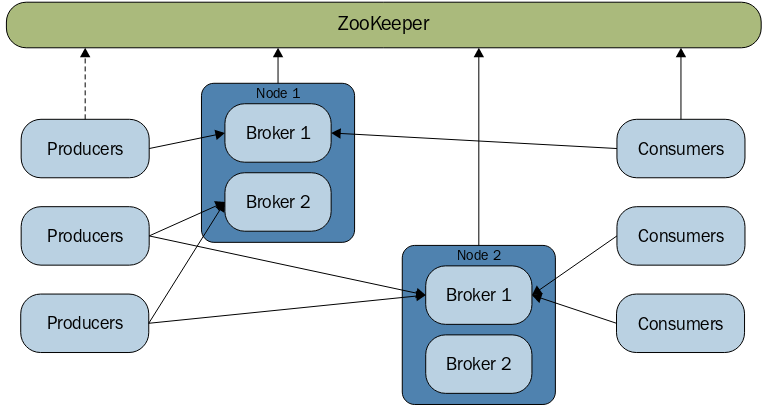
\includegraphics[keepaspectratio=true,scale=0.5]{img/kafka_multinode_multibroker}
    \caption{Multiple Broker / Multiple Node Kafka Cluster \cite{garg2013apache}}
  \label{fig:kafka_multinode_multibroker}
\end{figure}



\subsection{Mesos}
"Mesos is a cluster manager aiming for improved resource utilization by dynamically sharing resources among multiple frameworks " \cite{kakadia2015apache}.\\
The aim behind this framework is to provide a single platform which takes care of all hardware resources like CPU, memory, disk etc.
For the developer the whole cluster looks just like one big machine with cumulated resources.
This layer of abstraction makes it very easy to deploy and maintain applications running in a cluster.\\

According to mesos.apache.org \cite{apache_mesos}, there are some key features which make Mesos an attractive candidate as cluster manager for a big data stack like SMACK.
\begin{itemize}
    \item Linear scalability
        As proven by industrial application, scaling up to 10,000s of nodes is possible.
    \item High availability
        Zookeeper plays a key role when dealing with fault-tolerance, as the replicated master nodes use it to provide high availability.
        In addition it is possible to perform non-disruptive upgrades in the cluster.
    \item Containers
        Services like Docker run natively on Mesos.
    \item APIS
        There is a command-line tool to execute commands conveniently perform operations in the cluster, as well as a straight forward HTTP API to do requests programmatically.
    \item Cross Platform
        Mesos is supporting platforms like Linux, Windows, OSX and most cloud providers out of the box.
\end{itemize}

"In SMACK, Mesos orchestrates components and manages resources.
It is the secret for horizontal cluster scalation. ...
The equivalent in Hadoop is Apache Yarn" \cite{estrada2016big}.


\subsection{SMACK Stack}
Each SMACK technology for itself has proven to be robust and do an excellent job for the apsect it was designed for.
To build a big data architecture, we need frameworks which have connectors and can be easily put together to a powerful data pipeline.
Of course each of the technologies could be replaced by some other framework, but it has been shown, that those of SMACK are linkable very well \cite{estrada2016big}.\\
It is important to see, that SMACK focuses on \textit{fast data} and not necessarily only on \textit{big data}.
As the requirements of most modern large-scale applications demand processing in almost real-time, the need of such a stack is just the logical consequence.\\
"The SMACK stack emerges across verticals to help developers build applications to process fast data streams ...
The sole purpose of the SMACK stack is processing data in real time and outputting data analysis in the shortest possible time, which is usually in milliseconds" \cite{estrada2016big}.\\

Putting it together, Figure~\ref{fig:smack_stack} illustrates how the combination of Spark, Mesos, Akka, Cassandra and Spark could look like in a big data pipeline.
There are several users, endpoints or simply events which needs to be analyzed and processed.
While using Kafka producers to ingest the data, a consumer could directly be implemented in Spark using an available connector.
Storing the data in Cassandra is just a few lines of source code when using the Spark-Cassandra connector, which makes the pipeline easy to implement.
In this example the power of Akka is used to create a reactive application to give feedback to the users in a highly concurrent way and fault-tolerant by design.
Running all those frameworks on Mesos provides another layer of abstraction, so that the developer does not need to take care about the underlaying hardware and can let Mesos do its job as cluster manager.\\
This is just one of many possible setups for the stack.
The two applications used in this thesis to evaluate the results are described in more detail in Section~\ref{sec:evaluation_setup}.\\


\begin{figure}[!htbp]
  \centering
  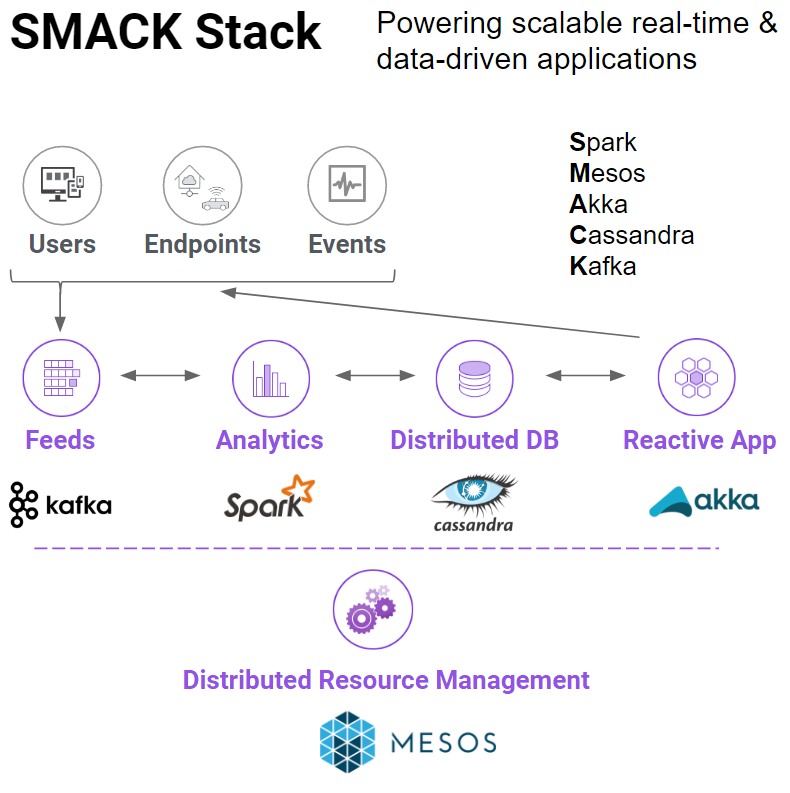
\includegraphics[keepaspectratio=true,scale=0.4]{img/smack_stack}
    \caption{SMACK Stack Illustration \cite{mesosphere}}
  \label{fig:smack_stack}
\end{figure}

\subsection{Reactive Systems}
Most modern applications have to fulfill high standards and many claim to be "reactive" systems.
The term "reactive system" is defined in the Reactive Manifesto \cite{reactive_manifesto}, where essentially four key factors have to be given to attribute an application as reactive:
\begin{enumerate}
    \item \textbf{Responsive}\\
          This attribute describes that the application has to respond in a defined time frame under all circumstances, as long as an answer can be given to the query.
          Without the definition of a time to response, it is not possible to determine whether an error occurred or not.
          Further fast response times improve user confidence and trust into the system and makes the whole application more interactive, which is highly desirable.
    \item \textbf{Resilient}\\
          Even in the event of hardware- or software faults, the system should stay intact and be able to respond to user queries.
          This is not only the case for highly critical applications but for any "reactive" system.
          The only way to achieve resilience, is to isolate components, use replication and delegate responsibilities.
          In case of an error only an isolated subsystem is affected and the supervising platform can recover this faulty component without affecting the whole application.
    \item \textbf{Elastic}\\
          Systems which are elastic stay responsive even under varying load.
          This means that the application can react to an increasing number of requests and still provide the required functionality even during peaks.
          The base for elasticity are these two key factors: replication and distribution of functionality.
          Elasticity also describes that if there are less requests than expected, the system can scale down and release resources which are not needed at the moment.
    \item \textbf{Message driven}\\
          The use of asynchronous messages is crucial to allow loose coupling and isolation of different components.
          The non-blocking nature of these messages lead to an efficient use of resources, as any component which is not receiving messages can stay idle and therefore does not consume CPU time.
          Further the explicit use of a message driven architecture allows to be independent of the location, as well as transparent scaling of components.
\end{enumerate}
The applications used in this thesis to evaluate strategies and the developed framework are reactive systems, which meet the criteria defined above.


\section{Thesis Organization}
In chapter \ref{ch:related}, related work can be found, including the comparison and summary of existing approaches.\\
Chapter \ref{ch:implementation} deals with the framework developed in the context of the thesis, including all its components.
Additionally there is an architecture overview, as well as the deployment diagram is discussed.
To give a deeper understanding of what is considered "interesting" for the framework when deciding which component to scale, the relevant metrics for each technology are discussed.
In chapter \ref{ch:evaluation} the evaluation and interpretation of the benchmark results can be found.
The experiment setup for the benchmark is described, including challenges and restrictions.
To give the reader a better understanding of the benchmark, a section about evaluation criteria and one about the significance of the benchmark is added to the chapter.
Further the setup, i.e. the applications used for the evaluation and the target architecture are described in this chapter.\\
The last chapter, \ref{ch:conclusion}, is about open issues, the conclusion itself and possible future work.

\section{Methodology}
The scientific approach used in this thesis comprises six parts.\\
In the first step, a literature review is performed and background information has to be gathered to serve as the theoretical background for this work, building on existing research.
After that an important part is the technology exploration.
In this step the individual parts of the SMACK-Stack have to be explored and knowledge about each technology is gathered.
In addition technical literature and reference books about the respective technologies can be read to get a better overview and a deeper understanding of each part of the SMACK stack.\\
The next step is the cloud setup, in which he whole stack is configured to be easily deployed.
One tool could be Amazon CloudFormation to provide a simple template for launching preconfigured instances.
Further various scripts have to be written to automate the deployment process an install required libraries, scripts and later on the applications to evaluate.\\
In the next step - the development - the framework to automatically redistribute and elastically scale the resources is implemented.
Further the two real world applications for the experiment benchmarks are implemented and extended to fit the needs of this thesis.
During the next step, namely the experiments, the scalability of the stack is determined by benchmarking individual configurations, where one application uses real world IoT data.\\
Then the performance of the stack under management of the developed framework is examined carefully.\\
In the last step the results are interpreted and the suggestions for how to distribute the resources are deduced and the corresponding reference deployment architecture and configuration is defined.
